% File SDSS2020_SampleExtendedAbstract.tex
\documentclass[10pt]{article}
\usepackage{sdss2020} % Uses Times Roman font (either newtx or times package)
\usepackage{url}
\usepackage{latexsym}
\usepackage{amsmath, amsthm, amsfonts}
\usepackage{algorithm, algorithmic}
\usepackage{graphicx}
\graphicspath{{images/}}
\title{Artificial Neural Networks and Deep Learning \\
Homework 1}

\author{
  Nicola Dean \\
  10617541 \\
  {\tt nicola.dean \\
  \tt @mail.polimi.it} \\\And
  Marco Fasanella \\
  10617541 \\
  {\tt marco.fasanella   \\
  \tt @mail.polimi.it}   \\\And
  Raffaello Fornasiere \\
    10617541 \\
    {\tt raffaello.fornasiere   \\
    \tt @mail.polimi.it}   \\\And
  Christian Spano \\
  10617541 \\
  {\tt christian.spano \\
  \tt @mail.polimi.it} \\}


\date{}

\begin{document}
\maketitle
\begin{abstract}
This document provides a basic template for the 2-page extended abstract
and some submission guidelines. The authors' names and affiliations should not be included. \footnote{Footnotes are also in smaller font.
See Table~\ref{fontsizes} for a list of font sizes.}
Including an abstract is optional, as the document itself is an extended abstract.
If included, an abstract should be a single paragraph.
\end{abstract}

{\bf Keywords:} VGG16, VGG19, Helpful

\section{Introduction}

We have based this SDSS template almost entirely on the template for
the annual conference of the Association for Computational Linguistics (ACL), whose
template includes the following paragraph of credits:
\begin{quotation}
\small % Okay to use \small inside quotation environment ONLY
This document has been adapted from the instructions for earlier ACL
proceedings, including those for ACL-2012 by Maggie Li and Michael
White, those from ACL-2010 by Jing-Shing Chang and Philipp Koehn,
those for ACL-2008 by Johanna D. Moore, Simone Teufel, James Allan,
and Sadaoki Furui, those for ACL-2005 by Hwee Tou Ng and Kemal
Oflazer, those for ACL-2002 by Eugene Charniak and Dekang Lin, and
earlier ACL and EACL formats. Those versions were written by several
people, including John Chen, Henry S. Thompson and Donald
Walker. Additional elements were taken from the formatting
instructions of the {\em International Joint Conference on Artificial
  Intelligence}.
\end{quotation}

\section{Methods}

In preparing the extended abstract,
we strongly encourage using the same four section headings seen here, namely,
Introduction, Methods, Data (or Results), and Discussion (or Conclusions).
Use of subsections is at the authors' discretion; see Section~\ref{info-on-sections}.

\subsection{Font Sizes and Layout}
Extended abstracts should be no more than two pages, including references,
in 10-point Times Roman font and two-column format, and must be submitted as pdf documents.
The \LaTeX\ template automatically uses the {\tt newtx} package if available
or {\tt times} if not to select Times Roman.
Please avoid changing the font size except, if desired, in the case of an extended
quotation as demonstrated above.

Both \LaTeX\ and
MS Word templates may be downloaded by visiting the conference website:
\begin{center}
\textbf{\texttt{github.com/SDSS2020/SDSS-templates}}
\end{center}
Margins should not be altered from those used in the template files.

\begin{table}[h]
\begin{center}
\begin{tabular}{|l|rl|}
\hline \bf Type of Text & \bf Font Size & \bf Style \\ \hline
paper title & 15 pt & bold \\
author names & 12 pt & bold \\
author affiliation & 12 pt & \\
the word ``Abstract'' & 12 pt & bold \\
section titles & 12 pt & bold \\
document text & 10 pt  &\\
captions & 10 pt & \\
abstract text & 10 pt & \\
bibliography & 10 pt & \\
footnotes & 9 pt & \\
\hline
\end{tabular}
\end{center}
\caption{\label{fontsizes} Sizes and styles of fonts used.}
\end{table}


\subsection{Sections}
\label{info-on-sections}

{\bf Headings}: While it is permissible to use bold print to introduce a paragraph
as seen here, please use the \verb+\section+,
\verb+\subsection+, and \verb+\subsubsection+
commands as in this \LaTeX\ document.  If you are using MS Word, please duplicate
the numbering and font-size conventions in this document.

\subsubsection{Numbering Sections}
As shown here, all sections, sub-sections, and sub-subsections are numbered.

\subsection{Citations}

In \LaTeX, please use the
{\tt sdss2020} bibliography style, as demonstrated by this example document.
MS Word users should duplicate the citation and reference section format seen here.

Citations within the text appear in parentheses
as~\cite{Nussbaum2018} or, if the author's name appears in the text
itself, as Nussbaum~\shortcite{Nussbaum2018}.  Treat double authors as
in~\cite{Wasserstein2016}, but write as in~\cite{Brunner} when more than two
authors are involved. Collapse multiple citations as
in~\cite{LaVange2019,Wasserstein2016}.  As alluded to above, full citations should not
be used as sentence constituents.  For instance, instead of
\begin{quote}
  ``\cite{Arbuthnot1710} found the first $p$-value ...''
\end{quote}
use
\begin{quote}
``Arbuthnot~\shortcite{Arbuthnot1710} found the first $p$-value ...''.
\end{quote}
Please make references complete, presentable, and
consistent. When using Bib\TeX, protect capital letters of names and
abbreviations in titles, as in \{B\}ayesian or \{EM\} algorithm,
in your .bib file.  For an example, notice that the ``FDA'' in
the title of \cite{LaVange2019} is typed as \verb+{FDA}+ in the .bib file
or else it would be incorrectly shown as ``fda'' in the references section.


\subsection{Footnotes}

{\bf Footnotes}: In \LaTeX, use the \verb+\footnote+
command\footnote{This is how a footnote should appear.}. If using
MS Word, please separate footnotes
from the text by a line\footnote{Note the line
separating the footnotes from the text.}.

\section{Data/Results}

We encourage the selective use of tables and/or figures as appropriate.

\subsection{Graphics and Tables}

Place figures and tables in the
paper near where they are first discussed, rather than at the end, if
possible.  It is acceptable that wide illustrations
may run across both columns.  The use of color
is allowed in extended abstract graphics.

\begin{figure}[ht]
\begin{center}
\centerline{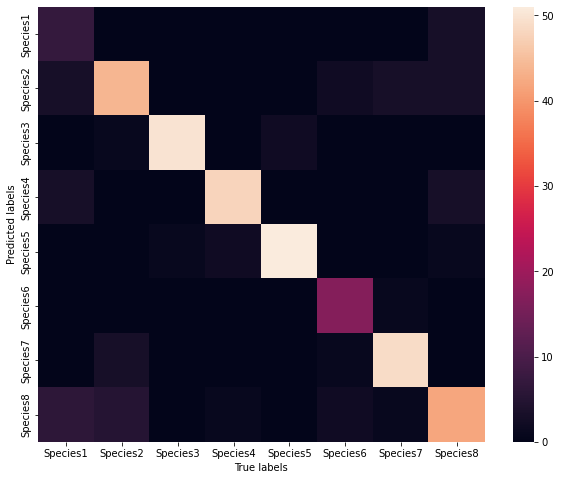
\includegraphics[width=\columnwidth]{VGG19_best}}
\caption{Ironically, Thomas Bayes was never asked to provide additional
simulation studies in the Results sections of his papers.}
\label{bayespic}
\end{center}
\end{figure}

\subsection{Captions}
Provide a caption below every figure and table; number each one
sequentially in the form shown in Figure~\ref{bayespic} and
Table~\ref{fontsizes}.

\section{Discussion/Conclusions}

\subsection{Appendices and Acknowledgements}

Please avoid the use of appendices and acknowledgements
as separate sections.  Any pertinent material should be included in the
body of the extended abstract rather than in an appendix.  If
acknowledgements are necessary, then they should be made using footnotes.

\subsection{Computer Code}

If you wish to provide links to accompanying code, this is allowable because
SDSS encourages best practices for reproducible research.  However, all
conclusions and exposition relevant to the refereeing process should appear in
the body of the extended abstract; furthermore, we cannot guarantee that
code will be checked or even consulted during the refereeing process.

\subsection{Refereeing Decisions}
The review is \textbf{anonymous}. Accepted papers must be presented in person at SDSS in St. Louis
from May 23 to 26, 2023.
Accepted papers' authors will be notified in plenty of time to make registration and travel
arrangements and for papers not accepted to submit a lightning abstract to the
conference if they so choose.

\bibliographystyle{sdss2020} % Please do not change the bibliography style
\bibliography{SampleReferencesForExtendedAbstract}

\end{document}
